\documentclass{article} % For LaTeX2e
\usepackage{nips14submit_e,times}
\usepackage{amsmath}
\usepackage{amsthm}
\usepackage{amssymb}
\usepackage{mathtools}
\usepackage{hyperref}
\usepackage{url}
\usepackage{algorithm}
\usepackage[noend]{algpseudocode}
%\documentstyle[nips14submit_09,times,art10]{article} % For LaTeX 2.09

\usepackage{graphicx}
\usepackage{caption}
\usepackage{subcaption}

\def\eQb#1\eQe{\begin{eqnarray*}#1\end{eqnarray*}}

\providecommand{\e}[1]{\ensuremath{\times 10^{#1}}}
\providecommand{\pb}[0]{\pagebreak}


\newenvironment{claim}[1]{\par\noindent\underline{Claim:}\space#1}{}
\newtheoremstyle{quest}{\topsep}{\topsep}{}{}{\bfseries}{}{ }{\thmname{#1}\thmnote{ #3}.}
\theoremstyle{quest}
\newtheorem*{definition}{Definition}
\newtheorem*{theorem}{Theorem}
\newtheorem*{question}{Question}
\newtheorem*{exercise}{Exercise}
\newtheorem*{challengeproblem}{Challenge Problem}
\newtheorem*{solution}{Solution}
\usepackage{verbatimbox}
\usepackage{listings}
\title{Intro to Macroeconmics: Problem Set II}


\author{
Youngduck Choi, Noah Gentile, Yuliya Takh \\
New York University \\
}


% The \author macro works with any number of authors. There are two commands
% used to separate the names and addresses of multiple authors: \And and \AND.
%
% Using \And between authors leaves it to \LaTeX{} to determine where to break
% the lines. Using \AND forces a linebreak at that point. So, if \LaTeX{}
% puts 3 of 4 authors names on the first line, and the last on the second
% line, try using \AND instead of \And before the third author name.

\newcommand{\fix}{\marginpar{FIX}}
\newcommand{\new}{\marginpar{NEW}}

\nipsfinalcopy % Uncomment for camera-ready version

\begin{document}


\maketitle

\begin{abstract}
This document contains the solutions to the problem set II.
\end{abstract}

\section{Solutions to the problems}

\begin{question}[1. Elasticity]
\end{question}
\begin{solution}
\textbf{(1)}
We first note that elasticity in general is defined by 
\eQb
\epsilon_{q,p} &=& \dfrac{\frac{\bigtriangleup q}{q}}{\frac{\bigtriangleup p}{p}}.
\eQe
The initial quantity, denoted as ${q_B}_{1}$, can be explicitly computed by
substituting the given values into the demand equation:
\eQb
{q_B}_{1} &=& 220 - 5(100) + \dfrac{1}{2}(1000) + 120 - 2(70), \\
&=& 200. 
\eQe
The new quantity demanded, denoted as ${q_B}_{2}$, can also be computed:
\eQb
{q_B}_{2} &=& 220 - 5(102) + \dfrac{1}{2}(1000) + 120 - 2(70), \\
&=& 190.
\eQe
Substituting the values into the elasticity equation, we have
\eQb
\epsilon_{q,p} &=& \dfrac{\frac{190-200}{200}}{\frac{102 - 100}{100}}, \\
&=& -\dfrac{5}{2}.
\eQe
Hence, the price-elasticity is $-2.5$.

\smallskip

\textbf{(2)}
The new quantity demanded can be computed as follows:
\eQb
{q_B}_{2} &=& 220 - 5(100) + \dfrac{1}{2}(1000) + 140 - 140 \\
&=& 220 
\eQe
Substituting the values into the elasticity equation, we have
\eQb
\epsilon_{q,p} &=& \dfrac{\frac{220-200}{200}}{\frac{140 - 120}{120}}, \\
&=& \dfrac{3}{5}.
\eQe
Hence, the cross-elasticity is $0.6$. As the cross-elasticity is positive,
Barro's and Mankiw's books are complements.

\pagebreak

\textbf{(3)}
The new quantity demanded can be computed as follows:
\eQb
{q_B}_{2} &=& 220 - 5(100) + \dfrac{1}{2}(1000) + 120 - 120 \\
&=& 220 
\eQe
Substituting the values into the elasticity equation, we have
\eQb
\epsilon_{q,p} &=& \dfrac{\frac{220-200}{200}}{\frac{60 - 70}{70}}, \\
&=& -\dfrac{3}{5}.
\eQe
Hence, the cross-elasticity is $-0.6$. As the cross-elasticity is negative, Barro's 
and the microeconomics books are complements.

\smallskip

\textbf{(4)}
The new quantity demanded can be computed as follows:
\eQb
{q_B}_{2} &=& 220 - 5(100) + \dfrac{1}{2}(1500) + 120 - 140 \\
&=& 470
\eQe
Substituting the values into the elasticity equation, we have
\eQb
\epsilon_{q,p} &=& \dfrac{\frac{470-200}{200}}{\frac{1500 - 1000}{1000}}, \\
&=& 2.7.
\eQe
Hence, the income elasticity is $2.7$. When income increases, the quantity 
demanded goes up, so it is a normal good.

\end{solution}

\bigskip

\begin{question}[2. Production]
\end{question}
\begin{solution}
\textbf{(1)}
We know that the Marginal Product of $L$ and of $K$ are respectively defined by
$\dfrac{\partial F}{\partial L } \> \text{ and } \> \dfrac{\partial F}{\partial K}.$ \\
Computing the above partials with the given production function, we obtain
\eQb
\dfrac{\partial F}{\partial L} &=& A, \\
\dfrac{\partial F}{\partial K} &=& B,
\eQe
where $A$ and $B$ are strictly positive constants.
Hence, the Marginal Product of $L$ is $A$ and the Marginal Product of $K$ is $B$.

\smallskip

\textbf{(2)}
With the above computation, we have shown that the marginal products are positive constants.
Hence, the marginal products are constants. It is decreasing, but not strictly decreasing.

\smallskip

\textbf{(3)}
The below figure contains the isoquants of production level 1 and 2 when $A = 2$ and $B = 5$.
\begin{figure}[h!]
  \caption{Isoquants of Production levels}
    \centering
  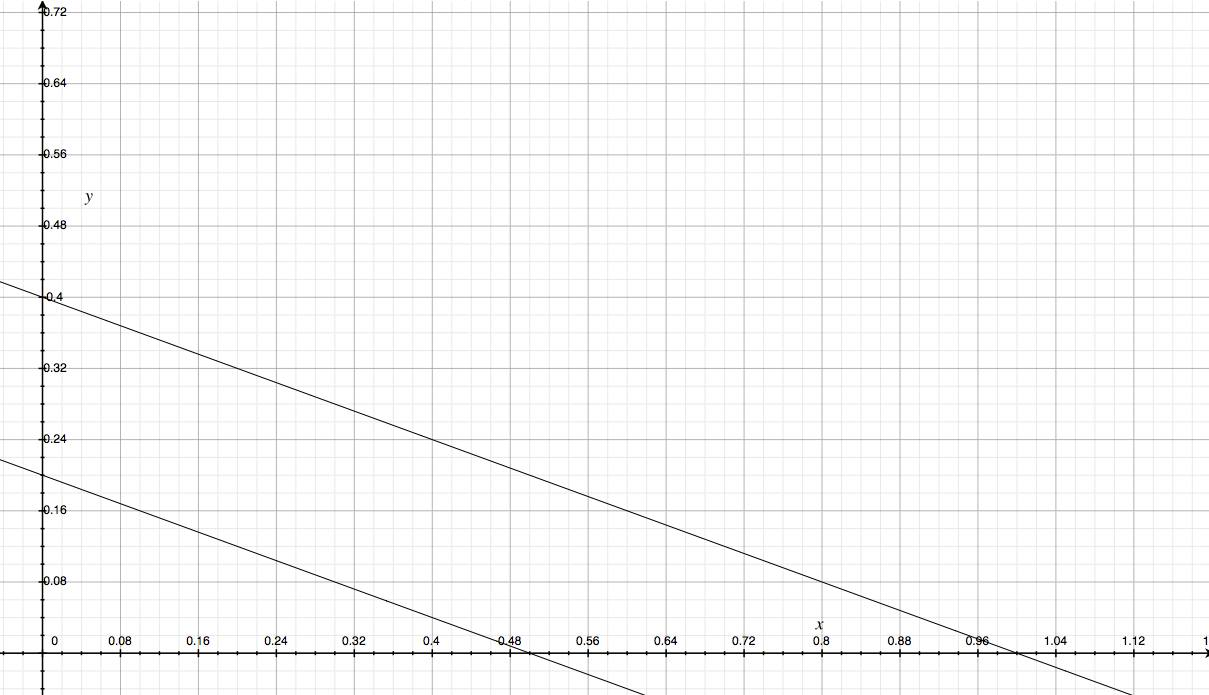
\includegraphics[width=0.5\textwidth]{iso.jpg}
\end{figure}

\end{solution}

\pagebreak

\begin{question}[3. The Impact of a Minimum Wage law]
\end{question}
\begin{solution}
\textbf{(1)}
We present the below figure, which depicts the labor market without a minimum wage and with minimum
wage together. The description inside the figure indicates the equilibrium wage and the equilibrium
number of employed people. The figure also is relevant for the number $2$.
\begin{figure}[h!]
  \caption{The labor market with and without a minimum wage \\ (a standard supply-and-demand diagram)}
    \centering
  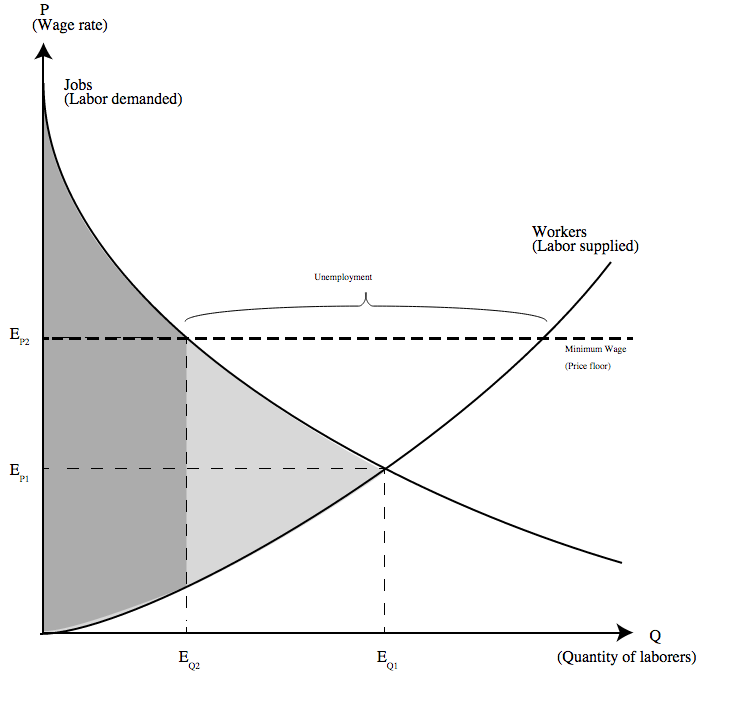
\includegraphics[width=0.85\textwidth]{graph3.jpg}
\end{figure}
\smallskip


\textbf{(2)}
Employment, decreased because the new quantity is less than the old equilibrium quantity. Plus Employers (demand curve) are willing to provide less jobs for the higher wage. Yes there is unemployment because the Workers (supply) want to be working more hours with the higher wage. But Employers have to reduce the amount of jobs available because of the higher wage. Thus you end up having a surplus of people not being able to attain jobs with this new wage. 

\pagebreak

\textbf{(3)}
Demand surplus decreases with the minimum wage law. Since the demand surplus is everything from the new wage to the demand curve, which has become smaller. Supply surplus increases due to the minimum wage laws. Since the supply surplus is everything from the new wage to where the supply curve is contained by the new quantity demanded. Which is a larger area. There is deadweight loss. This policy is not ready to an efficient outcome. Because in order to be efficient you need to have no deadweight loss, or as little as possible. This means that the quantity of jobs produced is less than the efficient one. With the wage law in place deadweight loss is increased from none to a larger quantity. Since there is a deadweight loss it means that resources were not allocated efficiently.

\end{solution}


\end{document}
